\documentclass[../../main.tex]{subfiles}

\graphicspath{{../../fig/}}
\setcounter{section}{0}

\begin{document}

\chapter{ニュートリノ振動}

本章では,本研究で開発する検出器が測定対象とする物理現象であるニュートリノ振動について述べる.

\section{素粒子標準模型におけるニュートリノ}

ニュートリノは中性子の$\beta$ 崩壊における電子のエネルギースペクトルが連続的であることを説明するために,1930年にW.Pauliによって提唱された粒子である\cite{intro:nupauli}.
ニュートリノが初めて観測されたのは1956年で、F.ReinesとC.L.Cowanが原子炉から放出された反電子ニュートリノの検出に成功した\cite{intro:reinescowan}.
その後,L.M.LedermanらのグループがAGS(Alternating Gradient Synchrotron)加速器を用いた実験で,パイ中間子の崩壊によって生じたミューニュートリノを検出した\cite{intro:reinescowan}.
1989年,欧州原子核研究機構(CERN)のLEP(Large Electron-Positron collider)で行われたZボソンの崩壊分岐比を調べる実験により,軽いニュートリノの世代数が3であることが示された\cite{intro:nu3gen}.
3世代目であるタウニュートリノは,2000年にDONUT(Direct Observation of NeUtrino Tau)実験において,タウニュートリノの散乱から生じるタウ粒子を原子核乾板により観測することで確かめられた\cite{intro:taunu}.

ニュートリノは素粒子標準模型に含まれる素粒子であり,電荷とカラー荷と持たないレプトンである.
ニュートリノは,標準模型に含まれる3つの相互作用(電磁相互作用,強い相互作用,弱い相互作用)のうち弱い相互作用しか作用せず,質量は0とされている.

\section{真空中のニュートリノ振動}
\label{intro:vacosci}
ニュートリノ振動とは,時間変化とともにニュートリノのフレーバーが変化するという物理現象であり,1962年に牧,中川,坂田によって提唱された\cite{intro:mns}.
ニュートリノ振動を説明するためには,ニュートリノが質量を持つことが必要条件になる.
1998年にスーパーカミオカンデ実験によってニュートリノ振動の存在が確実になった\cite{intro:SKneuosi}ことは,ニュートリノの質量を0とする標準模型の修正を迫る非常に重要な発見となった.

ニュートリノの質量固有状態を$\ket{\nu_{i}}\,(i=1,2,3)$,フレーバー固有状態を$\ket{\nu_{\alpha}}\,(\alpha=e,\mu,\tau)$とすると,フレーバー固有状態は質量固有状態の混合状態として次のように表される
\footnote{波動関数を$\nu_{\alpha}\equiv\bra{\nu_{\alpha}}\ket{\psi},\nu_{i}\equiv\bra{\nu_{i}}\ket{\psi}$とすると,
$\nu_{\alpha}=\sum_{i=1,2,3}U_{\alpha i}\nu_{i}$となる.}
:
\begin{gather}
  \label{intro:numix}
  \ket{\nu_{\alpha}}=\sum_{i=1,2,3}U^{*}_{\alpha i}\ket{\nu_{i}}
\end{gather}
ここで,$U_{\alpha i}$はPMNS(Pontecorvo-Maki-Nakagawa-Sakata)行列と呼ばれる$3\times3$のユニタリ行列である.
反ニュートリノの場合は以下のように表される:
\begin{gather}
  \label{intro:nubarmix}
  \ket{\bar{\nu}_{\alpha}}=\sum_{i=1,2,3}U_{\alpha i}\ket{\bar{\nu}_{i}}
\end{gather}
PMNS行列は一般に3つの混合角$\theta_{12},\theta_{23},\theta_{13}$および1つの複素位相角$\delta_{\mathrm{CP}}$によって次のようにパラメータ化される:
\begin{align}
  U &=
  \begin{pmatrix}
    1&0&0\\
    0&c_{23}&s_{23}\\
    0&-s_{23}&c_{23}\\
  \end{pmatrix}
  \begin{pmatrix}
  c_{13}&0&s_{13}e^{-i\delta_{\mathrm{CP}}}\\
  0&1&0\\
  -s_{13}e^{i\delta_{\mathrm{CP}}}&0&c_{13}\\
\end{pmatrix}
\begin{pmatrix}
  c_{12}&s_{12}&0\\
  -s_{12}&c_{12}&0\\
  0&0&1\\
\end{pmatrix}\nonumber\\
&=
\begin{pmatrix}
  c_{12}c_{13}&s_{12}c_{13}&s_{13}e^{-i\delta_{\mathrm{CP}}}\\
  -s_{12}c_{23} − c_{12}s_{23}s_{13}e^{i\delta_{\mathrm{CP}}}&c_{12}c_{23} - s_{12}s_{23}s_{13}e^{i\delta_{\mathrm{CP}}}&s_{23}c_{13}\\
  s_{12}s_{23} - c_{12}c_{23}s_{13}e^{i\delta_{\mathrm{CP}}}&-c_{12}s_{23} - s_{12}c_{23}s_{13}e^{i\delta_{\mathrm{CP}}}&c_{23}c_{13}\\
\end{pmatrix}
\label{eq:pmns}
\end{align}
ここで,$s_{ij}\equiv\sin{\theta_{ij}},c_{ij}\equiv\cos{\theta_{ij}}$である.$\delta_{\mathrm{CP}}\neq0,\pi$の場合,\eqref{intro:numix},\eqref{intro:nubarmix}より,ニュートリノと反ニュートリノとで混合に違いが生まれ,粒子と反粒子の対称性であるCP対称性の破れにつながる.そのため,$\delta_{\mathrm{CP}}$はCP位相角と呼ばれる.

質量固有状態$\ket{\nu_{i}}$の時刻0から時刻$t$への時間発展は,平面波を仮定すると,エネルギー$E_{i}$,運動量$\vb*{p}_{i}$を用いて次のように書ける:
\begin{gather}
  \ket{\nu_{i}(t)}=e^{-i\left(E_{i}t-\vb*{p}_{i}\cdot\vb*{x}\right)}\ket{\nu_{i}(0)}
\end{gather}
ここで,自然単位系を用いている(以後同様).
ニュートリノは相対論的粒子であるから,その質量が運動量の大きさに比べて十分小さいという近似$\left|\vb*{p}_{i}\right|\gg m_{i}$を用いると,
\begin{gather}
  E_{i}=\sqrt{\left|\vb*{p}_{i}\right|^{2}+m_{i}^{2}}\simeq\left|\vb*{p}_{i}\right|+\frac{m_{i}^{2}}{2\left|\vb*{p}_{i}\right|}\simeq\left|\vb*{p}_{i}\right|+\frac{m_{i}^{2}}{2E}
\end{gather}
となる.また,ニュートリノの速さはほぼ光速$c$であるから,ニュートリノの飛行距離を$L$とすると,$t\simeq L$である.
よって,質量固有状態が距離$L$飛行した後の状態は,
\begin{gather}
  \ket{\nu_{i}(L)}=e^{-i\frac{m_{i}^{2}L}{2E}}\ket{\nu_{i}(0)}
\end{gather}
と書ける.
したがって,$L=0$においてフレーバー固有状態$\ket{\nu_{\alpha}}=\sum_{i}U^{*}_{\alpha i}\ket{\nu_{i}}$であったニュートリノが,距離$L$飛行した後の状態は,
\begin{align}
  \ket{\nu_{\alpha}(L)}
  &=\sum_{i}U^{*}_{\alpha i}\ket{\nu_{i}(L)}\nonumber\\
  &=\sum_{i}U^{*}_{\alpha i}e^{-i\frac{m_{i}^{2}L}{2E}}\ket{\nu_{i}}
\end{align}
となるから,$L=0$においてフレーバー固有状態$\ket{\nu_{\alpha}}$であったニュートリノが,距離$L$飛行した後にフレーバー固有状態$\ket{\nu_{\beta}}$で観測される確率$P\left(\nu_{\alpha}\rightarrow\nu_{\beta}\right)$は,
\begin{align}
  P\left(\nu_{\alpha}\rightarrow\nu_{\beta}\right)
  &=\left|\bra{\nu_{\beta}} \ket{\nu_{\alpha}(L)}\right|^2\nonumber\\
  &=\left|\sum_{i,j}U_{\beta j}U^{*}_{\alpha i}e^{-i\frac{m_{i}^{2}L}{2E}}\bra{\nu_{j}}\ket{\nu_{i}}\right|^2\nonumber\\
  &=\left|\sum_{i}U_{\beta i}U^{*}_{\alpha i}e^{-i\frac{m_{i}^{2}L}{2E}}\right|^2\nonumber\\
  &=\sum_{i,j}U_{\beta i}U^{*}_{\alpha i}U^{*}_{\beta j}U_{\alpha j}e^{-i\frac{\left(m_{i}^{2}-m_{j}^{2}\right)L}{2E}}\nonumber\\
  &=\sum_{i,j}\Omega^{\alpha\beta}_{ij}e^{-i\frac{\Delta m_{ij}^{2}L}{2E}}
\end{align}
となる.ここで,$\Omega^{\alpha\beta}_{ij}\equiv U_{\beta i}U^{*}_{\alpha i}U^{*}_{\beta j}U_{\alpha j},\Delta m_{ij}^{2}\equiv m_{i}^{2}-m_{j}^{2}$と定義した.さらに計算を進めると,
\begin{align}
  \label{intro:oscillationformula}
  P\left(\nu_{\alpha}\rightarrow\nu_{\beta}\right)
  &=\sum_{i=j}\Omega^{\alpha\beta}_{ij}+\sum_{i>j}\left(\Omega^{\alpha\beta}_{ij}e^{-i\frac{\Delta m_{ij}^{2}L}{2E}}+\left(\Omega^{\alpha\beta}_{ij}\right)^{*}e^{i\frac{\Delta m_{ij}^{2}L}{2E}}\right)\nonumber\\
  &=\sum_{i=j}\Omega^{\alpha\beta}_{ij}+2\sum_{i>j}\mathrm{Re}\left[\Omega^{\alpha\beta}_{ij}\right]\cos\left(\frac{\Delta m_{ij}^{2}L}{2E}\right)+2\sum_{i>j}\mathrm{Im}\left[\Omega^{\alpha\beta}_{ij}\right]\sin\left(\frac{\Delta m_{ij}^{2}L}{2E}\right)\nonumber\\
  &=\sum_{i=j}\Omega^{\alpha\beta}_{ij}+2\sum_{i>j}\mathrm{Re}\left[\Omega^{\alpha\beta}_{ij}\right]\left\{1-2\sin^{2}\left(\frac{\Delta m_{ij}^{2}L}{4E}\right)\right\}+2\sum_{i>j}\mathrm{Im}\left[\Omega^{\alpha\beta}_{ij}\right]\sin\left(\frac{\Delta m_{ij}^{2}L}{2E}\right)\nonumber\\
  &=\sum_{i=j}\Omega^{\alpha\beta}_{ij}+2\sum_{i>j}\mathrm{Re}\left[\Omega^{\alpha\beta}_{ij}\right]\left\{1-2\sin^{2}\left(\frac{\Delta m_{ij}^{2}L}{4E}\right)\right\}+2\sum_{i>j}\mathrm{Im}\left[\Omega^{\alpha\beta}_{ij}\right]\sin\left(\frac{\Delta m_{ij}^{2}L}{2E}\right)\nonumber\\
  &=\sum_{i,j}\Omega^{\alpha\beta}_{ij}-4\sum_{i>j}\mathrm{Re}\left[\Omega^{\alpha\beta}_{ij}\right]\sin^{2}\left(\frac{\Delta m_{ij}^{2}L}{4E}\right)+2\sum_{i>j}\mathrm{Im}\left[\Omega^{\alpha\beta}_{ij}\right]\sin\left(\frac{\Delta m_{ij}^{2}L}{2E}\right)\nonumber\\
  &=\delta_{\alpha\beta}-4\sum_{i>j}\mathrm{Re}\left[\Omega^{\alpha\beta}_{ij}\right]\sin^{2}\left(\frac{\Delta m_{ij}^{2}L}{4E}\right)+2\sum_{i>j}\mathrm{Im}\left[\Omega^{\alpha\beta}_{ij}\right]\sin\left(\frac{\Delta m_{ij}^{2}L}{2E}\right)
\end{align}
となる.したがって,\eqref{intro:oscillationformula}の第2,3項が消えない条件を考えると,ニュートリノ振動が生じるための必要十分条件は,ニュートリノが異なる質量固有値を持ち($\Delta m_{ij}^{2}\neq0$),かつフレーバー混合が存在する(PMNS行列$U$の非対角成分が0でない)ことである.
反ニュートリノについての振動確率$P\left(\bar{\nu}_{\alpha}\rightarrow\bar{\nu}_{\beta}\right)$については,\eqref{intro:numix},\eqref{intro:nubarmix}から,PMNS行列の複素共役を取ったものを考えればよく,\eqref{intro:oscillationformula}の第3項の符号が反転する.

\section{物質効果}

\ref{intro:vacosci}節では真空中でのニュートリノ振動を考えたが,実際には,物質中を運動するニュートリノは周囲の物質との弱い相互作用によりポテンシャル・エネルギーを得るため,ニュートリノ振動にも変化が生じる.
この効果を物質効果と呼ぶ.
この効果は1978年にL.Wolfensteinにより定式化され\cite{intro:MSWwolfenstein},1985年にはS.P.MikheyevとA.Yu.Smirnovが物質効果を太陽ニュートリノに適用し,仮に混合角が小さくてもニュートリノ振動の遷移確率を十分大きくすることが可能であることを示した\cite{intro:MSWsmirnov}.
物質効果は以上3人の名前の頭文字を取ってMSW効果と呼ばれることもある.

ニュートリノと物質(電子)の相互作用のうち,$Z$ボソンの交換により相互作用する中性カレント反応は全フレーバーに対して生じるので,ニュートリノ振動には効かない.
一方,$W$ボソンの交換により相互作用する荷電カレント反応は,電子ニュートリノのみが電子と反応するため,それによるポテンシャル・エネルギー
\begin{align}
  V(x)=\sqrt{2}G_{F}N_e(x)
\end{align}
を付加的に獲得する.ここで,$G_{F}$はフェルミ結合定数,$N_e(x)$は物質中の電子の数密度である.

\section{ニュートリノ振動実験とその最新結果}

\begin{figure}[htbp]
  \centering
  \makebox[\textwidth][c]{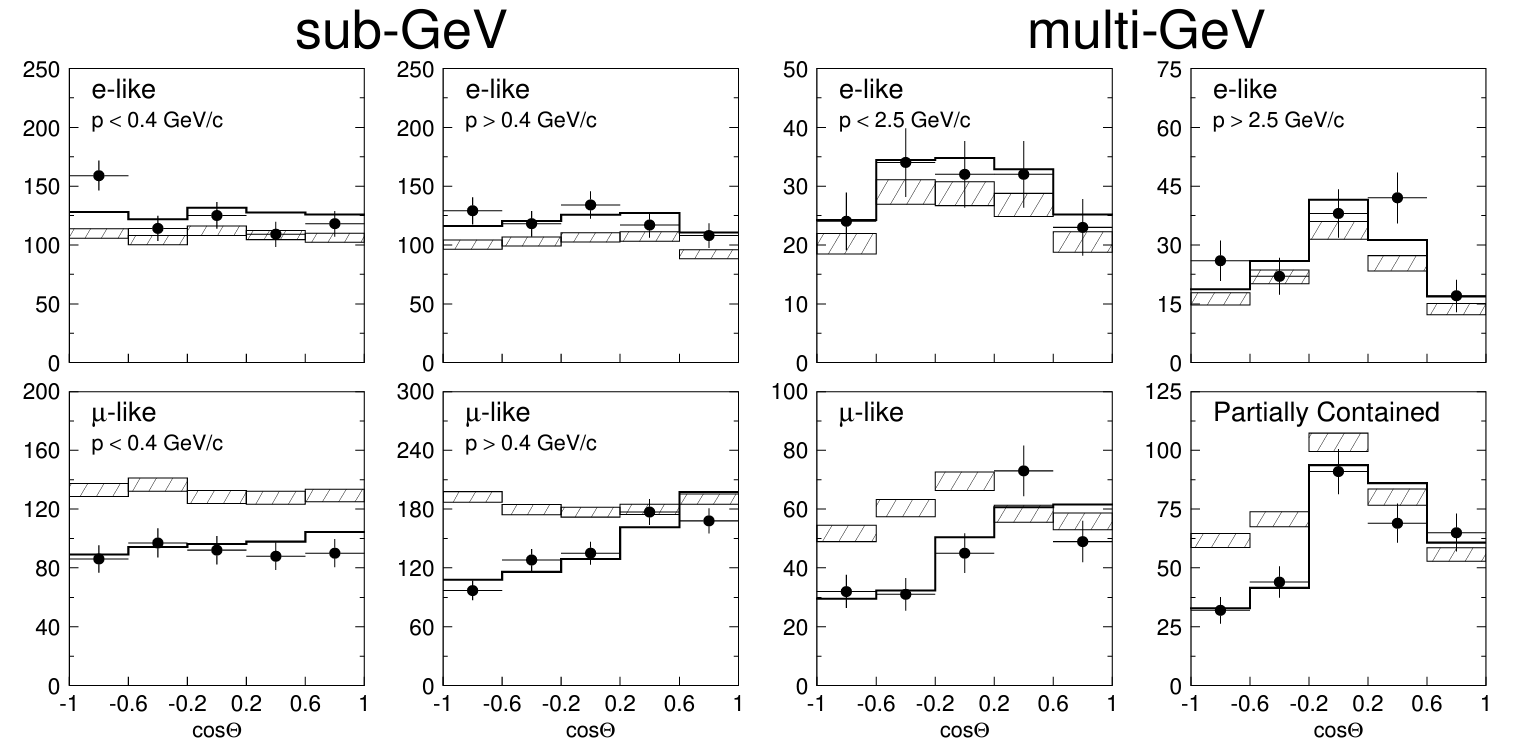
\includegraphics[width=1.0\textwidth]{intro/SKneutrinoosc.png}}
  \caption[スーパーカミオカンデで観測された大気ニュートリノの天頂角分布]{スーパーカミオカンデで観測された大気ニュートリノの天頂角分布\cite{intro:SKneuosi}.斜線部の領域はニュートリノ振動がない時の予想値を表し,黒線はニュートリノ振動を仮定した時のベストフィットを表している.$\nu_{\mu}$の事象数(図中で"$\mu$-like"と記載)がニュートリノ振動を仮定しないときに比べて少ないことが分かる.}
  \label{fig:intro:SKneutrinoosc}
\end{figure}

1968年,Homestake実験は初めて太陽ニュートリノ$\nu_{e}$を観測したが,観測されたニュートリノの数が標準太陽模型の予言値の1/3しかなかった\cite{intro:Homestake}.
その後,カミオカンデ実験やSAGE(Soviet-American Gallium Experiment),GALLEX(GALLium EXperiment)でも太陽ニュートリノの事象数が標準太陽模型の予言値よりも有意に小さいことを報告した\cite{intro:kamiokande}\cite{intro:SAGE}\cite{intro:GALLEX}.
この問題は「太陽ニュートリノ問題」として長年の謎であった.
その解決の鍵となったのがニュートリノ振動である.

ニュートリノ振動は,1998年に初めてスーパーカミオカンデによって観測された\cite{intro:SKneuosi}.
スーパーカミオカンデで観測された大気ニュートリノの天頂角分布を求めたところ,特に地球の裏側から貫通してくる($\cos\theta<0$)ような$\nu_{\mu}$の事象数がニュートリノ振動がない時に予想される事象数より小さいことが分かり,これがニュートリノ振動によって説明できることが確認された(図\ref{fig:intro:SKneutrinoosc}).

2001年には,SNO(Sudbury Neutrino Observatory)実験の$\nu_e$だけでなく3世代全てのニュートリノに感度をもつ重水を用いた測定により,実際に$\nu_{e}\rightarrow\nu_{\mu},\nu_{\tau}$の遷移が起きていることが確かめられ,太陽ニュートリノ問題は解決に至った\cite{intro:SNO}.

それぞれのニュートリノ振動パラメータの測定方法について以下に述べる.
また,現在のニュートリノ振動パラメータの測定結果を表\ref{intro:tab:osciparames}に示す.
\begin{itemize}
  \item $\theta_{12}$, $\Delta m^2_{21}$
  
  スーパーカミオカンデ実験やSNO実験による太陽ニュートリノやKamLAND(Kamioka Liquid scintillator Anti-Neutrino Detector)実験の原子炉ニュートリノによる$\nu_{e}(\bar{\nu}_e)$の生存確率によって測定されている.基線$L$が数百kmの場合,生存確率は,
  \begin{align}
    P(\nu_e\rightarrow\nu_{e})\approx 1-\sin^{2}2\theta_{12}\sin^{2}\left(\frac{\Delta m^{2}_{21}L}{4E}\right)
  \end{align}
  となり($P(\bar{\nu}_e\rightarrow\bar{\nu}_{e})$も同じ式),$\theta_{12}$, $\Delta m^2_{21}$が測定される.
  また,太陽ニュートリノの物質効果によって,$\Delta m^2_{21}$は符号も含めて測定されている.
  
  \item $\theta_{23}$, $|\Delta m^2_{32}|$
  
  スーパーカミオカンデにおける大気ニュートリノ振動の実験やT2K(Tokai to Kamioka)実験,NO$\nu$A(NuMI Off-axis $\nu_{e}$ Appearance)実験などの長基線加速器ニュートリノ振動実験によって$\nu_{\mu}$の消失事象から測定されている.$\nu_{\mu}$の生存確率は,$\theta_{13}\approx0$として,
  \begin{align}
    P(\nu_{\mu}\rightarrow\nu_{\mu})\approx 1-\sin^{2}2\theta_{23}\sin^{2}\left(\frac{\Delta m^{2}_{32}L}{4E}\right)
  \end{align}
  となり,$\theta_{23}$, $|\Delta m^2_{32}|$が測定される.
  
  \item $\theta_{13}$
  
  T2K実験やNO$\nu$A実験などの加速器ニュートリノ実験やDaya-Bay実験などの原子炉ニュートリノ実験により精密に測定される.
  基線$L$が数kmの中基線原子炉ニュートリノ実験の場合,$\bar{\nu}_{e}$の生存確率は,
  \begin{align}
    P(\bar{\nu}_e\rightarrow\bar{\nu}_{e})\approx 1-\sin^{2}2\theta_{13}\sin^{2}\left(\frac{\Delta m^{2}_{31}L}{4E}\right)
  \end{align}
  となり,$\theta_{13}$が測定される.
  現在,最も精度良く測定されている.
  
  \item $\delta_{\mathrm{CP}}$
  
  $\nu_{\mu}$から$\nu_{e}$への振動確率と$\bar{\nu}_{\mu}$から$\bar{\nu}_{e}$への振動確率の差をとることによって,
  \begin{align}
    &P(\bar{\nu}_{\mu}\rightarrow\bar{\nu}_{e})-P(\nu_{\mu}\rightarrow\nu_{e})\nonumber\\
    &=2\sin2\theta_{12}\sin2\theta_{23}\sin2\theta_{13}\cos\theta_{13}\sin\delta_{\mathrm{CP}}\sin\left(\frac{\Delta m^{2}_{21}L}{4E}\right)\sin\left(\frac{\Delta m^{2}_{32}L}{4E}\right)\sin\left(\frac{\Delta m^{2}_{31}L}{4E}\right)
  \end{align}
  となり,$\delta_{\mathrm{CP}}$の寄与する項のみを測定することができる.
  しかし,実際には,ニュートリノと反ニュートリノでは物質効果に差があることによりCP非対称性に似た紛らわしい効果が生じるため,注意を要する.
  
\end{itemize}

\begin{table}[h]
  \centering
  \caption[現在のニュートリノ振動パラメータの測定値]{現在のニュートリノ振動パラメータの現在の測定値\cite{intro:oscipara}.表中の値はbest-fit$\pm1\sigma~(3\sigma$ range)である. \label{intro:tab:osciparames}}
  \begin{tabular}{ccc} \hline
    ニュートリノ振動パラメータ & 順階層 & 逆階層 \\ \hline \hline
    $\Delta m^2_{21}~[\times10^{-5}~\mathrm{eV^2}]$ & $7.36^{+0.16}_{-0.15}~(6.93\rightarrow7.93)$ &  $7.36^{+0.16}_{-0.15}~(6.93\rightarrow7.93)$\\ \hline
    $\Delta m^2_{32}~[\times10^{-3}~\mathrm{eV^2}]$ & $2.448^{+0.023}_{-0.031}~(2.367\rightarrow2.521)$ & $-2.492^{+0.025}_{-0.030}~(-2.578\rightarrow-2.413)$\\ \hline
    $\sin^2\theta_{12}~[10^{-1}]$ & $3.03^{+0.13}_{-0.13}~(2.63\rightarrow3.45)$ & $3.03^{+0.13}_{-0.13}~(2.63\rightarrow3.45)$\\ \hline
    $\sin^2\theta_{23}~[10^{-1}]$ & $4.55^{+0.18}_{-0.15}~(4.16\rightarrow5.99)$ & $5.69^{+0.13}_{-0.21}~(4.17\rightarrow6.06)$\\ \hline
    $\sin^2\theta_{13}~[10^{-2}]$ & $2.23^{+0.07}_{-0.06}~(2.04\rightarrow2.44)$ & $2.23^{+0.06}_{-0.06}~(2.03\rightarrow2.45)$ \\ \hline
    $\delta_{\mathrm{CP}}/\pi$ & $1.24^{+0.18}_{-0.13}~(0.77\rightarrow1.97)$ & $1.52^{+0.14}_{-0.15}~(1.07\rightarrow1.90)$\\ \hline
  \end{tabular}
\end{table}

\section{ニュートリノ振動における未解決問題}

現在,未解決のまま残っているニュートリノ振動における問題として,以下のようなものがある.
\begin{itemize}
  \item ニュートリノのCP対称性の破れ
  
  $\delta_{\mathrm{CP}}\neq0,\pi$であれば,PMNS行列に複素成分が現れ,CP対称性の破れにつながる.
  現在,T2K実験が90\%の有意度で$\delta_{\mathrm{CP}}\neq0,\pi$であることを示唆している\cite{intro:t2k2023}が,未だ決定には至っていない.
  
  ビッグバン宇宙論によると,宇宙誕生時では粒子と反粒子が同数作られたと考えられているが,現在の我々の宇宙にはほとんど粒子から構成される物質しか存在しない.
  この粒子と反粒子の非対称性を説明するには,Sakharovの3条件と呼ばれる(1)バリオン数の破れ,(2)CおよびCP対称性の破れ,(3)熱平衡の破れが必要である\cite{intro:sakhanov}.
  このうち,(1)と(3)を満たす過程が存在することは分かっているが,(2)については,すでに測定されているクォークのCP対称性の破れだけでは不十分なことが分かっている.
  そこで,レプトンにおけるCP対称性の破れが注目されており,それはニュートリノと反ニュートリノの振動確率の違いを見ることによって調べられる.
  $\delta_{\mathrm{CP}}\neq0,\pi$であることが確かめられれば粒子と反粒子の非対称性の謎を解決する手がかりとなるため,精密な測定が求められている.
  
  \item 質量階層性問題
  
  $\Delta m^2_{32}$の絶対値は測定されているが,その正負は分かっていない.
  それは,ニュートリノ振動確率の支配的な項に$\sin^2\left(\frac{\Delta m^2_{32}L}{4E}\right)$の形で現れるからである.
  $\Delta m^2_{32}$の符号に応じて,$m_1<m_2<m_3$となる順階層と$m_3<m_1<m_2$となる逆階層の2通りの質量階層性が考えられている.
  $\Delta m^2_{21}$と同様に,物質効果を用いて$\Delta m^2_{32}$の符号を調べることができる.
  例えば,地球の裏側から通過してくる大気ニュートリノが地球から受ける物質効果を調べる方法があるが,太陽ニュートリノの場合と比べるとその効果は小さく,質量階層性の決定に未だ至っていない.
  
  \item $\theta_{23}$のオクタント問題
  
  表\ref{intro:tab:osciparames}から分かるように,現在測定されている$\theta_{23}$の値は,最大混合$\theta_{23}=45^{\circ}$に近い.
  最大混合の場合,レプトンの世代間において新たな対称性の存在が示唆されている\cite{intro:octant}.
  
\end{itemize}

\end{document}